\documentclass{scrartcl}
%packages we're using. Filled with a default set
\usepackage[ngerman]{babel}
\usepackage[utf8]{inputenc}
\usepackage{amsmath}
\usepackage{amsfonts}
\usepackage{amssymb}
\usepackage{listings}
\usepackage{multirow}
\usepackage{tikz}
\usepackage{graphicx}
\usepackage{setspace}
\usepackage{float}
\usepackage{microtype}
\usepackage{url}
\usepackage{times}
\usetikzlibrary{calc,through,backgrounds,shapes}

% intended for defining things like% \newcommand{\ml}[1]{$\mathbb{#1}$}
\newcommand{\fun}[1]{\texttt{#1}} %I'm dired of writing...

\title{ETI GP 5 - SS 2012}
\date{\today}
\author{Philip Becker, Thomas Breier, Matthias Brugger, Jakob Buchgraber,\\Dominik Durner, Julius Michaelis, Nils Kunze, Simon Wimmer}



\begin{document}

\maketitle
\tableofcontents
\newpage

\section{TODO}
- alphabetische Sortierung der Terminology. \\
- Namen aufm titel zu lang \\
- Rechtschreibprüfung \\
- Absätze, neue Seiten etc sinnvoll verteilen \\

\section{Terminology} \begin{description}

\item[Debuggee]
	The piece of software for which we want to analyze cache usage. The term debuggee is used because it’s run with valgrind which is usually used for debugging.
\item[Matrix]
	A matrix is, in our case, an area of the memory which the debuggee has marked to contain data that is to be analyzed by our software. 
\item [Access]
	An access is an event generated for the debuggee. It marks loading or storing data to the main memory with a specific address.
\item[Relative Access]
	We are matching memory accesses to matrices and compute coordinates from that. For each access and it's previous access, a difference is coputed, and that is called a relative access. \newline
	\begin{tikzpicture} %Tikzpictures are going to be fun. Our coordinate systems diverge...
		\draw [color=gray] (-0.5,-0.5) grid (1.5,1.5);
		\node (frst) at (1,0) {}; %nth access
		\node (scnd) at (0,1) {}; %n+1-th access
		\draw [->,color=green,thick] (frst) -- (scnd) node [midway,right,draw=none] {$(-1,-1)$};
	\end{tikzpicture}
\item[Pattern]
	A pattern is an ordered set of relative accesses. These accesses have been observed subsequently multiple (to be exact: at least two) times. It is not guaranteed that the first access of a pattern always occures first. Patterns can't tell you anything about when or in which compositions they occur
\item[Sequence]
	When scanning for patterns in the access stream, a series of consecutive accesses is often accounted to one pattern. The length of this series and what happens next is bundled into a sequence.
\end{description}

\section{Examples} In this section, we will look at some applications of ETIS. ETIS is designed for the analysis of programs which operate on matrices. We will therefore look at some of these matrix problems and different algorithms solving them, which vary in the order and frequency of memory accesses. Most importantly, we will show how to modify a sample program so as to be able to analyze it with ETIS.

\subsubsection*{Notes}
\begin{itemize}
\item As the examples presented here do not focus on the solution of the problem itself but should only briefly illustrate how to use ETIS in practice, we make assumptions and simplifications in our models and do not treat every possible solution approach in full detail.

\item When claiming that ETIS reveals a difference in cache usage, we assume significantly large matrices.

\item The code snippets in this section are written in C. We do not provide entire correct programs but concentrate on the relevant algorithmic parts, leaving out procedures and variable declarations if their function is clear from the context.

\item In the notation \texttt{a[i][j]}, the index \texttt{i} denotes the row (in the first dimension) and \texttt{j} denotes the column (in the second dimension).
\end{itemize}


\subsection{Applications of ETIS}

A typical problem where ETIS can help the programmer is solving (partial) differential equations in two dimensions with iterative methods. We will look at a very simplified model of the distribution of heat, e.g. in a metal plate.
As we cannot simulate the distribution for every point on the plate, we discretize the problem, obtaining a grid which can be represented by a matrix. The boundary values are invariant throughout the entire simulation process. We assume that the heat value for an inner node is the mean of the four adjoining nodes (which are either inner nodes or nodes on the boundary). The inner values are iteratively computed using a red-black scheme as marked in the following picture (we assume a $5 \times 5$ matrix):

\begin{figure}[h]
\begin{tikzpicture} [scale=0.8,font=\footnotesize]
	\fill [gray!15] (-2,-2) rectangle +(1,5);
	\fill [gray!15] (2,-2) rectangle +(1,5);
	\fill [gray!15] (-2,-2) rectangle +(5,1);
	\fill [gray!15] (-2,2) rectangle +(5,1);
	\draw [step=1cm,gray] (-2,-2) grid ++(5,5);
	
	\fill [color=red] (.5,.5) circle [radius=.125cm];
	\fill [color=red] (-.5,-.5) circle [radius=.125cm];
	\fill [color=red] (-.5,1.5) circle [radius=.125cm];
	\fill [color=red] (1.5,1.5) circle [radius=.125cm];
	\fill [color=red] (1.5,-.5) circle [radius=.125cm];
	\fill [color=black] (-.5,.5) circle [radius=.125cm];
	\fill [color=black] (.5,1.5) circle [radius=.125cm];
	\fill [color=black] (.5,-.5) circle [radius=.125cm];
	\fill [color=black] (1.5,.5) circle [radius=.125cm];
	
	\node at (-1.5,2.5) {$v$};
	\node at (-.5,2.5) {$v$};
	\node at (.5,2.5) {$v$};
	\node at (1.5,2.5) {$v$};
	\node at (2.5,2.5) {$v$};
	\node at (2.5,1.5) {$v$};
	\node at (2.5,.5) {$v$};
	\node at (2.5,-.5) {$v$};
	\node at (2.5,-1.5) {$v$};
	\node at (1.5,-1.5) {$v$};
	\node at (.5,-1.5) {$v$};
	\node at (-.5,-1.5) {$v$};
	\node at (-1.5,-1.5) {$v$};
	\node at (-1.5,-.5) {$v$};
	\node at (-1.5,.5) {$v$};
	\node at (-1.5,1.5) {$v$};
	
	% 
	\node (offset) at (6,0) {};
	\draw [step=1cm,gray] (-1.25+6,-1.25) grid ++(3.5,3.5);
	
	\fill [red] (.5,.5) +(offset) circle [radius=.125cm] node [above] {$(i,j)$};
	\fill [red] (-.5,-.5) +(offset) circle [radius=.125cm];
	\fill [red] (-.5,1.5) +(offset) circle [radius=.125cm];
	\fill [red] (1.5,1.5) +(offset) circle [radius=.125cm];
	\fill [red] (1.5,-.5) +(offset) circle [radius=.125cm];
	\fill [black] (-.5,.5) +(offset) circle [radius=.125cm] node [left] {$(i,j-1)$};
	\fill [black] (.5,1.5) +(offset) circle [radius=.125cm] node [above] {$(i-1,j)$};
	\fill [black] (.5,-.5) +(offset) circle [radius=.125cm] node [above] {$(i+1,j)$};
	\fill [black] (1.5,.5) +(offset) circle [radius=.125cm] node [right] {$(i,j+1)$};
\end{tikzpicture}
\end{figure}

One iteration consists of an update of all black nodes and an update of all red nodes. Thus we can implement the updates in one iteration as follows:
\begin{lstlisting}
// update inner black nodes
for(i=1; i<N-1; i++)
   for(j=1+(i%2); j<N-1; j+=2)
      m[i][j] = ( m[i-1][j] + m[i+1][j] 
                + m[i][j-1] + m[i][j+1] )/4.0;

// update inner red nodes
for(i=1; i<N-1; i++)
  for(j=1+((i+1)%2); j<N-1; j+=2)
      m[i][j] = ( m[i-1][j] + m[i+1][j] 
                + m[i][j-1] + m[i][j+1] )/4.0;
\end{lstlisting}
In the above implementation, all the red or black nodes in one row are updated before we jump to the next row. Alternatively, we could update the nodes by columns. Whether updates by columns instead of updates by rows make any difference can be decided with the help of ETIS. Furthermore, ETIS can visualize the access patterns; in this example, one obvious pattern consists of the four accesses to the adjoining matrix entries (in a fixed order).

Another very similar example is the following Jacobi method, where we use two grids/matrices $A$ and $B$ instead of the red-black update order (only parts of the two grids are depicted):
\begin{figure}[h]
\begin{tikzpicture} [font=\footnotesize]
	\draw [step=1cm,gray] (-1.25,-1.25) grid ++(3.5,3.5);
	
	\fill [blue] (.5,.5) circle [radius=.125cm] node [above] {$a_{i,j}$};
	\fill [gray] (-.5,-.5) circle [radius=.125cm];
	\fill [gray] (-.5,1.5) circle [radius=.125cm];
	\fill [gray] (1.5,1.5) circle [radius=.125cm];
	\fill [gray] (1.5,-.5) circle [radius=.125cm];
	\fill [red] (-.5,.5) circle [radius=.125cm] node [above] {$a_{i,j-1}$};
	\fill [red] (.5,1.5) circle [radius=.125cm] node [above] {$a_{i-1,j}$};
	\fill [red] (.5,-.5) circle [radius=.125cm] node [above] {$a_{i+1,j}$};
	\fill [red] (1.5,.5) circle [radius=.125cm] node [above] {$a_{i,j+1}$};
	
	\node (offset) at (5,0) {};
	\draw [step=1cm,gray] (-1.25+5,-1.25) grid ++(3.5,3.5);
	
	\fill [red] (.5,.5) +(offset) circle [radius=.125cm] node [above] {$b_{i,j}$};
	\fill [gray] (-.5,-.5) +(offset) circle [radius=.125cm];
	\fill [gray] (-.5,1.5) +(offset) circle [radius=.125cm];
	\fill [gray] (1.5,1.5) +(offset) circle [radius=.125cm];
	\fill [gray] (1.5,-.5) +(offset) circle [radius=.125cm];
	\fill [blue] (-.5,.5) +(offset) circle [radius=.125cm] node [above] {$b_{i,j-1}$};
	\fill [blue] (.5,1.5) +(offset) circle [radius=.125cm] node [above] {$b_{i-1,j}$};
	\fill [blue] (.5,-.5) +(offset) circle [radius=.125cm] node [above] {$b_{i+1,j}$};
	\fill [blue] (1.5,.5) +(offset) circle [radius=.125cm] node [above] {$b_{i,j+1}$};
	
	\node [font=\large] at (.5,2.5) {$A$};
	\node [font=\large] at (.5+5,2.5) {$B$};
\end{tikzpicture}
\end{figure}
\\$A$ is the input and output grid, i.e. $A$ is initialized with the initial values and contains the final computed values at the end of the iterations. A naive method could look like this: In one iteration, the entries of $B$ are updated first, using the values in $A$ (marked \textcolor{red}{red}), then $A$ is updated using the (updated) entries from $B$ (marked \textcolor{blue}{blue}):
\begin{lstlisting}
for(i=1; i<N-1; i++)
for(j=1; j<N-1; j++)
   b[i][j] = ( a[i-1][j] + a[i][j-1] 
             + a[i+1][j] + a[i][j+1] )/4.0;

for(i=1; i<N-1; i++)
for(j=1; j<N-1; j++)
   a[i][j] = ( b[i-1][j] + b[i][j-1] 
             + b[i+1][j] + b[i][j+1] )/4.0;
\end{lstlisting}
However, ETIS will reveal that other update methods are more efficient in terms of cache usage: For example, we could first update the minimal number of rows in $B$ until we can update the next row in $A$ which has not been updated yet in the current iteration. Then we move on to the next not-yet-updated row in $B$ etc. The advantage of such an "'interwoven"' update method is that after having updated the rows in $B$, the respective values are still available in the cache memory, so when updating the row in $A$ in the next step, we do not need to load the necessary values of $B$ in the cache again.

We will look at yet another example: We want to compare different implementations of multiplying two square matrices. Let $A$ and $B$ denote the operand matrices and $C$ the product matrix, then we can naively implement the multiplication $C=A \cdot B$ as follows (\texttt{N}-by-\texttt{N} matrices):
\begin{lstlisting}
for(i=0; i<N; i++)
   for(j=0; j<N; j++)
      for(k=0; k<N; k++)
         c[i][j] += a[i][k] * b[k][j];
\end{lstlisting}
The three nested loops can be permutated without changing the result, thus we obtain 6 simple versions of this matrix multiplication algorithm. One could argue that traversing the matrices by rows is more cache-efficient than a traversal by columns as a two-dimensional matrix is stored linearly - row after row - in memory. Thus we can reduce the number of cache loads by ensuring that both $A$ and $B$ are traversed by rows (whereas in the above example $B$ is traversed by columns). The idea is to multiply $A$ not by $B$ but by the transpose of the transpose of $B$, which is mathematically the same:
\begin{lstlisting}
// compute bt = transpose of b
for(i=0; i<N; i++)
   for(j=0; j<N; j++)
      for(k=0; k<N; k++)
         c[i][j] += a[i][k] * bt[j][k];
\end{lstlisting}
Obviously, the index \texttt{k} traverses both operand matrices by rows.

To outline further approaches, there is the possibility to multiply $A$ and $B$ blockwise. Blocking can be done in one or two dimensions, which means that the index range of either one of the inner loops is split into equal intervals (called "'blocks"') or both inner loops are split. (There is no point in using blocking for the outer loop too as the outer index is always the one which changes least.)


\subsection{Preparing a Sample Program for Analysis with ETIS}

Suppose we have a square matrix \texttt{a} of size \texttt{M} $\times$ \texttt{N} which we want to trace, then the following code snippet will tell ETIS to record and analyze all accesses to the memory area where \texttt{a} is stored:
\begin{lstlisting}
SSIM_MATRIX_TRACING_START(a, M, N, sizeof(double), "a");
// ... (crucial matrix accesses that are to trace)
SSIM_MATRIX_TRACING_STOP(a);
\end{lstlisting}
The commands in lines 1 and 3 are so-called \emph{Valgrind client requests}, by means of which the sample program can communicate with ETIS (or the underlying Valgrind tools, respectively). The syntax of these requests is as follows:

\begin{lstlisting} [numbers=none]
SSIM_MATRIX_TRACING_START(void* addr, int m, int n, 
                          size_t ele_size, char* name);
\end{lstlisting}
signals the beginning of a trace of all accesses on the memory area starting at address \texttt{addr} representing a \texttt{m}-by-\texttt{n} matrix with entries of size \texttt{ele\_size}. When tracing multiple matrices, the argument \texttt{name} should be a unique identifier for the traced matrix, as the ETIS user interface will display the specified name for each traced matrix.
With the request
\begin{lstlisting} [numbers=none]
SSIM_MATRIX_TRACING_STOP(void* addr);
\end{lstlisting}
you can stop the recording of accesses on the referenced matrix.

Valgrind client requests for starting and stopping the tracing must be submitted for each matrix.

\subsubsection*{Comparing multiple implementations}
For the problems in the previous examples, there were different solution approaches. Each of these can be encapsuled in a method of its own. Suppose we have the two methods
\begin{lstlisting} [numbers=none]
void method1(double* a) { /* ... */ }
void method2(double* a) { /* ... */ }
\end{lstlisting}
which solve a certain problem on a \texttt{N}-by-\texttt{N} matrix \texttt{a}; then we have to use the requests once for each method:
\begin{lstlisting}
init(a); // initializes the entries of a
SSIM_MATRIX_TRACING_START(a, N, N, sizeof(double), 
                          "method1 - a");
method1(a);
SSIM_MATRIX_TRACING_STOP(a);

SSIM_FLUSH_CACHE;
init(a);
SSIM_MATRIX_TRACING_START(a, N, N, sizeof(double), 
                          "method2 - a");
method2(a);
SSIM_MATRIX_TRACING_STOP(a);
\end{lstlisting}
As both methods operate on the same matrix, calling \texttt{method2} directly after \texttt{method1} (and after the repeated initialization) could distort the memory access statistics if the cache still holds some matrix entries that are later used again in \texttt{method2}. (We assume that the \texttt{init} procedure does not flush the cache or resets all matrix entries.) Therefore we need to flush the entire cache in between the two method calls in line 7, which can be done via another Valgrind client request:
\begin{lstlisting} [numbers=none]
SSIM_FLUSH_CACHE;
\end{lstlisting}

\subsubsection*{Further implementation notes}
If you have many alternative implementations which have the same method signature, it may prove useful to define a function pointer to such an implemented method and use that in generic function calls. This makes the different methods exchangable and comparable.

\section{Mctracer} \subsection{Call hierarchy: Memory access}

\tikzstyle{accarrw} = [draw,->,thick, shorten <=10, shorten >=10]
\tikzstyle{trmain} = [draw,fill=red!50]
\tikzstyle{trsim} = [draw,fill=green!50]
\tikzstyle{trstats} = [draw,fill=blue!50]
\tikzstyle{trseq} = [draw,fill=purple!50]
\begin{tikzpicture}[scale=0.9]
	\node [trmain]  (instrument) at (0,2.5) {\fun{mt\_instrument}};
	\node [trmain]  (fE) at (0,1.5)         {\fun{flushEvents}};
	\node [cloud,draw,aspect=2,cloud puffs=9] (magic) at (0,0.25) {magic};
	\node [trsim]   (load) at (2,-1)        {\fun{ssim\_load}} node [trsim] (store) at (-2,-1) {\fun{ssim\_store}};
	\node [trstats] (ums)  at (0,-2)        {\fun{update\_matrix\_stats}};
	\node [trstats] (fm)   at (5,-1.5)      {\fun{find\_matrix}};
	\node [trsim]   (cr)   at (5,-2.5)      {\fun{cache\_ref}};
	\node [trsim]   (csr)  at (6,-3.5)      {\fun{cache\_setref}};
	\node [trstats] (umas) at (0,-3)        {\fun{update\_matrix\_access\_stats}};
	\node [trseq]   (umps) at (0,-4)        {\fun{update\_matrix\_pattern\_stats}};
	\node [trseq]   (ppb)  at (0,-6)        {\fun{process\_pattern\_buffer}};
	\node [trseq]   (sec)  at (-4.5,-8)       {\fun{subpatttern\_elimination\_check}};
	\node [trseq]   (mpf)  at (-5.25,-7)    {\fun{mark\_pattern\_findings}};
	\node [trseq]   (dap)  at (2.5,-8)      {\fun{delete\_access\_pattern}};
	\node [trseq]   (fnp)  at (0,-7)        {\fun{find\_new\_patterns}};
	\node [trseq]   (fs)   at (5.1,-7)        {\fun{find\_sequences}};
	\node [trseq]   (rapa) at (5.1,-9)        {\fun{reallocate\_sequencearray}};
	\foreach \s/\e in {instrument/fE, load/ums, store/ums, ums/fm, ums/cr, cr/csr, ums/umas, umas/umps, ppb/mpf, ppb/fnp, ppb/fs, fs/rapa}{
		\path [->,thick,draw] (\s) -- (\e);
	}
	\foreach \s/\e in {sec/mpf, sec/dap, fnp/sec, fnp/dap, fE/magic.north east, fE/magic.north west, magic.south west/store, magic.south east/load}{
		\path [->,thick,draw,dashed] (\s) -- (\e);
	}
	\draw (-7.25,-8.5) rectangle (-1,-12.75);
	\path [->,thick,draw,dashed] (umps) -- (ppb) node [midway,right,draw,xshift=0.5em] {When the buffer is full};
	\path [->,thick,draw]        (-7,-9) -- (-6,-9) node [right] {Call, always};
	\path [->,thick,draw,dashed] (-7,-9.5) -- (-6,-9.5) node [right] {Call, conditional};
	\node [anchor=west,trmain]  at(-7,-10.5)   {Method from \texttt{tr\_main.c}};
	\node [anchor=west,trsim]   at(-7,-11.1) {Method from \texttt{tr\_sim.c}};
	\node [anchor=west,trstats] at(-7,-11.7) {Method from \texttt{tr\_stats.c}};
	\node [anchor=west,trseq]   at(-7,-12.3) {Method from \texttt{tr\_sequences.c}};
\end{tikzpicture}

\subsection{Explanation by Methods}

\begin{description} %the plan is to add a longer description to the more complex ones of these
\item[\fun{cache\_ref()}] Maps an access to one or two cache sets. Queries \fun{cache\_setref} to return hit or miss.
\item[\fun{cache\_setref()}] For a given cache set and adress: Updates the set and returns hit or miss;
\item[\fun{ssim\_load()}] Proxy function for calling \fun{update\_matrix\_stats(..., MATRIX\_LOAD)}
\item[\fun{ssim\_store()}] Proxy function for calling \fun{update\_matrix\_stats(..., MATRIX\_STORE)}
\item[\fun{find\_matrix()}] Finds the matrix containing a given address
\item[\fun{update\_matrix\_stats()}] For the given address: Updates the absolute position access stats
\item[\fun{update\_matrix\_access\_stats()}] For the given matrix and absolute access: updates the relative access statistics
\item[\fun{update\_matrix\_pattern\_stats()}] Fills the buffer for pattern recognition with one relative access per call. Invokes \fun{process\_pattern\_buffer} when full.
\item[\fun{process\_pattern\_buffer()}] Management function for pattern/sequence recognition. Keeps a buffer stating which access belongs to which pattern. Invokes marking existing patterns in that buffer, finding new patterns and the statistics on that buffer
\item[\fun{process\_pattern\_buffer()}] For a matrix, one of it's patterns and it's access buffer: Marks each location that pattern occurs
\item[\fun{mark\_pattern\_findings()}] For a matrix and it's access buffer: Tries to find non-marked, short, repeating patterns. Avoids/deletes patterns being parts of other patterns
\item[\fun{subpatttern\_elimination\_check()}] For a pattern: Eliminates it, if it is part ("subpattern") of any other pattern of that matrix
\item[\fun{delete\_access\_pattern}] Eleminates the given pattern. Makes sure to clean all remains
\item[\fun{find\_sequences}] The workhorse of the pattern/sequence statistics. Counts hits and misses for the accesses in the patterns. Sums up the length of repetitions of paterns as sequences
\item[\fun{reallocate\_sequencearray}] Helper to make sure enough space is reserved for the current number of sequences

\end{description}

\section{File Format} \subsection{Introduction}

Firstly I'd like to state that we are closely following the GZIP file format specification version 4.3 (as found at http://www.gzip.org/zlib/rfc-gzip.html) in structure, design and sometimes content.

\paragraph{Purpose}

The purpose of this specification is to define a byte-oriented data format that can save all of the statistical data collected by the valgrind tool McTracer. Specifically that means that it's able to save
the data collected for several diffrent matrices into one file. The data for one matrix consists of information about individual matrix elements, relative accesses, access patterns and access sequences as
well as some statistical data about the matrix as a whole.

\paragraph{Intended audience}

This specification is intended for use by implementors of software to read the etis format and display it in a way that makes it easier to understand by humans.

The text of the specification assumes a background in programming at the level of bits and other primitve data representations.

\paragraph{Changes from previous versions}
Currently we are at Version 3. Version 1 was bascially a draft, outlining the ideas behind the format for the first time. Version 2 improved the general design and made changes to some field-sizes. 
In Version 3 support for patterns and sequences was added.

\newpage
\subsection{Detailed Specification} \subsubsection{Overall conventions}

In the diagrams below, a box like this:
\begin{verbatim}
+---+
|   | <-- the vertical bars might be missing
+---+
\end{verbatim}
represents one byte; a box like this:
\begin{verbatim}
+==============+
|              |
+==============+
\end{verbatim}
represents a variable number of bytes.

Within a computer, a number may occupy multiple bytes. All multi-byte numbers in the format described here are 
stored with the least-significant byte first (at the lower memory address). For example, the decimal number 520 
is stored as:
\begin{verbatim}
    0        1
+--------+--------+
|00001000|00000010|
+--------+--------+
 ^        ^
 |        |
 |        + more significant byte = 2 x 256
 + less significant byte = 8
\end{verbatim}

All values are unsigned unless noted otherwise.

\subsubsection{File Format}

An etis file consists of a file-header, a cluster of matrice-headers and a number of matrix data blocks (MDB). 
The header formats and the format of the MDBs will be specified in the following sections.

\paragraph{File-Header (FH) 4 Byte}$\;$ \\

The file header has the following structure:

\begin{verbatim}
+---+---+---+---+
|ID1|ID2| V |NM |
+---+---+---+---+
\end{verbatim}
ID1 (IDentification 1) 1 Byte \\
ID2 (IDentification 2) 1 Byte
\begin{addmargin}[0,5cm]{0,5cm} 
	These have fixed values ID1 = 175 (0xaf, \textbackslash0257), ID2 = 254 (0xfe, \textbackslash0376), to identify the file as being in etis format.
\end{addmargin} 
V (Version) 1 Byte
\begin{addmargin}[0,5cm]{0,5cm} 
	Specifies the version of the fileformat that the current file is in. Currently at 3.
\end{addmargin}
NM (Number of Matrices) 1 Byte
\begin{addmargin}[0,5cm]{0,5cm} 
	The overall number of traced matrices.
\end{addmargin}

\paragraph{Matrix Header (MH) 36 Byte}$\;$ \\

Exactly FH:NM matrix header simply appear one after another in the file, with no additional information 
before, between, or after them.
\begin{verbatim}
+---+---+---+---+---+---+---+---+---+---+---+---+---+---+---+---+
|  SX   |  SY   |NLA|NSA|NAP|NSQ|              ADR              |
+---+---+---+---+---+---+---+---+---+---+---+---+---+---+---+---+
|     MDBADR    |     SLH       |      SLM      |      SSH      |
+---+---+---+---+---+---+---+---+---+---+---+---+---+---+---+---+
|      SSM      |
+---+---+---+---+
\end{verbatim}
SX (Size X) 2 Byte (signed!)
\begin{addmargin}[0,5cm]{0,5cm} 
	The size of the matrix in x direction (number of columns). Must be positive.
\end{addmargin}
SY (Size Y) 2 Byte (signed!)
\begin{addmargin}[0,5cm]{0,5cm} 
	The size of the matrix in y direction (number of rows). Must be positive.
\end{addmargin}
NLA (Number of Loading Accesses) 1 Byte
\begin{addmargin}[0,5cm]{0,5cm} 
	The number of saved relative accesses loading data from this matrix. Maximum of eight.
\end{addmargin}
NSA (Number of Storing Accesses) 1 Byte
\begin{addmargin}[0,5cm]{0,5cm} 
	The number of saved relative accesses storing data into this matrix. Maximum of eight.
\end{addmargin}
NAP (Number of Accesss Patterns) 1 Byte
\begin{addmargin}[0,5cm]{0,5cm} 
	The number of access patterns saved for this matrix.
\end{addmargin}
NSQ (Number of access SeQuences) 1 Byte
\begin{addmargin}[0,5cm]{0,5cm} 
	The number of access sequences saved for this matrix.
\end{addmargin}
ADR (ADRess) 8 Byte $\rightarrow$ 64-Bit
\begin{addmargin}[0,5cm]{0,5cm} 
	The pointer of the matrix.
\end{addmargin}
MDBADR (MDB ADRess) 4 Byte
\begin{addmargin}[0,5cm]{0,5cm} 
	The adress of the affiliated MDB in this file.
\end{addmargin}
SLH (Sum Load Hits) 4 Byte
\begin{addmargin}[0,5cm]{0,5cm} 
	The sum of all load hits for this matrix.
\end{addmargin}
SLM (Sum Load Misses) 4 Byte
\begin{addmargin}[0,5cm]{0,5cm} 
	The sum of all load misses for this matrix.
\end{addmargin}
SSH (Sum Store Hits) 4 Byte
\begin{addmargin}[0,5cm]{0,5cm} 
	The sum of all store hits for this matrix.
\end{addmargin}
SSM (Sum Store Misses) 4 Byte
\begin{addmargin}[0,5cm]{0,5cm}
	The sum of all store misses for this matrix.
\end{addmargin}

\paragraph{Matrix Data Block (MDB)}$\;$ \\

A Matrix Data Block consists of two byte arrays, some (MH:NLA+MH:NSA) relative accesses, some (MH:NAP) access 
patterns, several (MH:NSQ) access sequences and the name assigned to the matrix.

\subparagraph{2 x Byte Array (BA) (MH:SX * MH:SY) Byte}$\;$ \\

One byte array has a size of MH:SX*MH:SY and every byte signifies one matrix element. The matrix is traversed 
row by row. The first byte array represents the tracked load accesses, the second one the store accesses. 
The value of each byte signifies the hit to miss ratio of accesses to the specific element. 
A value of 0 signifies 0\% hits (only misses) and a value of 254 signifies 100\% hits. 
The value 255 is reserved to show that there wasn't any access to this element.

\subparagraph{Relative Access (RA) 12 Byte}$\;$ \\

First there are all MH:NLA diffrent relative accesses for loading from the matrix, then the MH:NSA diffrent 
relative accesses for storing into the matrix. They simply appear one after another in the file, with no 
additional information before, between, or after them.
\begin{verbatim}
+---+---+---+---+---+---+---+---+---+---+---+---+
|  OX   |  OY   |      SH       |      SM       |
+---+---+---+---+---+---+---+---+---+---+---+---+
\end{verbatim}
OX (Offset X) 2 Byte (signed!)
\begin{addmargin}[0,5cm]{0,5cm} 
	The x offset of this relative access.
\end{addmargin}
OY (Offset Y) 2 Byte (signed!)
\begin{addmargin}[0,5cm]{0,5cm} 
	The y offset of this relative access.
\end{addmargin}
SH (Sum of Hits) 4 Byte
\begin{addmargin}[0,5cm]{0,5cm} 
	The accumulated number of hits for this type of relative access.
\end{addmargin}
SM (Sum of Misses) 4 Byte
\begin{addmargin}[0,5cm]{0,5cm} 
	The accumulated number of misses for this type of relative access.
\end{addmargin}
\newpage
\subparagraph{Access Pattern (AP) 7 Byte + AP:LEN * 12 Byte}$\;$ \\

An access pattern combines a series of relative accesses. There are exactly MH:NAP diffrent access patterns
 one after another. Each pattern consists of a short pattern header and afterwards AP:LEN diffrent relative 
accesses as defined above. They simply appear one after another in the file, with no additional information 
before, between, or after them.
\begin{verbatim}
+---+---+---+---+---+---+---+
|ID |      SO       |  LEN  |
+---+---+---+---+---+---+---+
\end{verbatim}
ID (IDentification) 1 Byte
\begin{addmargin}[0,5cm]{0,5cm} 
	An identification number that is unique in the context of the current matrix.
\end{addmargin}
SO (Sum of Occurences) 4 Byte
\begin{addmargin}[0,5cm]{0,5cm} 
	The accumulated sum of occurences of this pattern.
\end{addmargin}
LEN (LENgth) 2 Byte
\begin{addmargin}[0,5cm]{0,5cm} 
	The length of this pattern.
\end{addmargin}
	
\subparagraph{Access Sequence (SQ) 12 Byte}$\;$ \\

An access sequence consists of uninterrupted repetitions of a pattern combined with the next access or next 
pattern. There are exactly MH:NSQ diffrent sequences one after another. They simply appear one after another 
in the file, with no additional information before, between, or after them.
\begin{verbatim}
+---+---+---+---+---+---+---+---+---+---+---+---+
|PID|      SO      |   RP   |  NX   |  NY   |NID|
+---+---+---+---+---+---+---+---+---+---+---+---+
\end{verbatim}
PID (Pattern IDentification) 1 Byte
\begin{addmargin}[0,5cm]{0,5cm} 
	The AP:ID of the pattern that is repeated.
\end{addmargin}
SO (Sum of Occurences) 4 Byte
\begin{addmargin}[0,5cm]{0,5cm} 
	The accumulated sum of occurrences of this sequences
\end{addmargin}
RP (RePetitions) 2 Byte
\begin{addmargin}[0,5cm]{0,5cm} 
	The number of uninterrupted repetitions of the pattern.
\end{addmargin}
NX (Next access offset X) 2 Byte (signed!)
\begin{addmargin}[0,5cm]{0,5cm} 
	The x offset of the access following the sequence.
\end{addmargin}
NY (Next access offset Y) 2 Byte (signed!)
\begin{addmargin}[0,5cm]{0,5cm} 
	The y offset of the access following the sequence.
\end{addmargin}
NID (Next IDentification) 1 Byte
\begin{addmargin}[0,5cm]{0,5cm} 
	References the pattern following the sequence. 0xff if none could be found.
\end{addmargin}

\subparagraph{Name (NA)}$\;$ \\
\begin{verbatim}
+========+
|  NAME  |
+========+
\end{verbatim}
NAME (Name) Null terminated
\begin{addmargin}[0,5cm]{0,5cm} 
	The name of the matrix, as it's passed when the tracing starts. ASCII-encoded.
\end{addmargin}

\subsection{Overview}
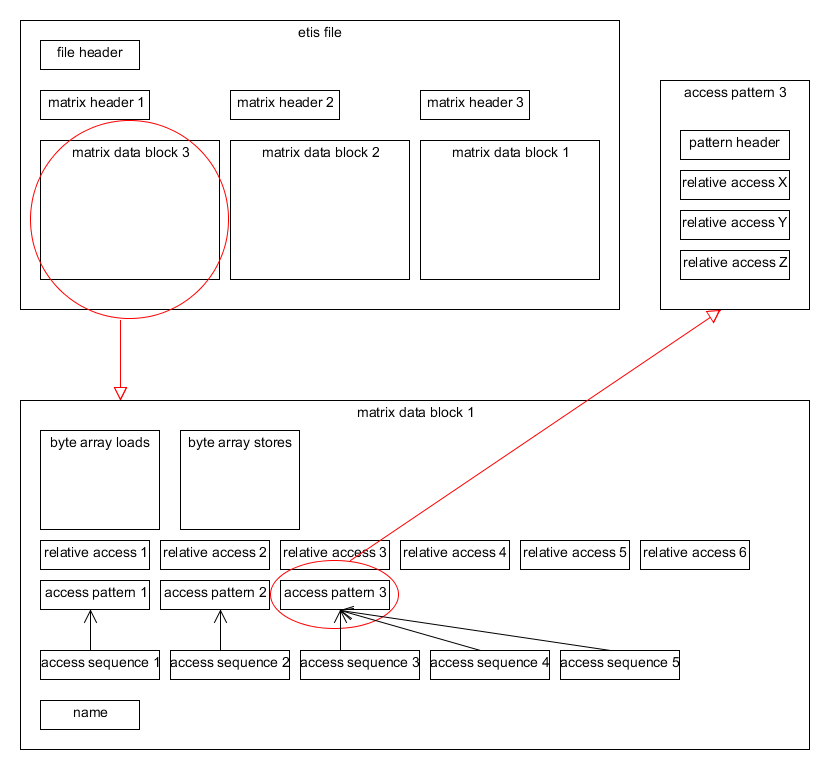
\includegraphics[width=\textwidth]{fileformat/structure}
This is a conceptual outline of an etis file. It consists of the file header, three matrix headers and three matrix data blocks (MDB). The first MDB is then displayed in more detail to show the different element
that it contains, namely namely two byte arrays, several relative accesses, three patterns with one, one and three sequences and the name. The last detail shows an access pattern in some more detail.

\section{GUI} \subsection{Basic Structure} The GUI is implemented solely in Java, utilizing the Swing Architecture. The project is structured according to the Model–View–Controller pattern. It consists of three packages (\texttt{data}, \texttt{view} and \texttt{controller}), separating the data from the interface, connected through the \texttt{controller}. The package \texttt{data} is responsible for reading the data files and providing a comprehensive interface to retrieve the data. The package \texttt{view} is responsible for displaying the data to the user. It communicates with the data only via the \texttt{controller} (and vice versa). Therefore the \texttt{controller}'s purpose is to manage the entire data flow of the software. It sends requested data to the user interface or requests new data to be loaded from a file. 

\subsection{Class Responsibilities - Package \texttt{view}}
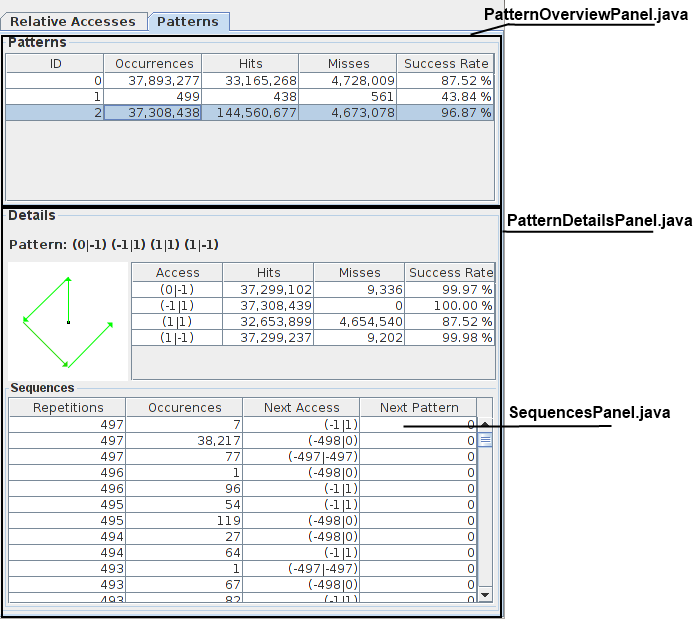
\includegraphics[width=350px]{gui/classresp2.png}
\newpage 
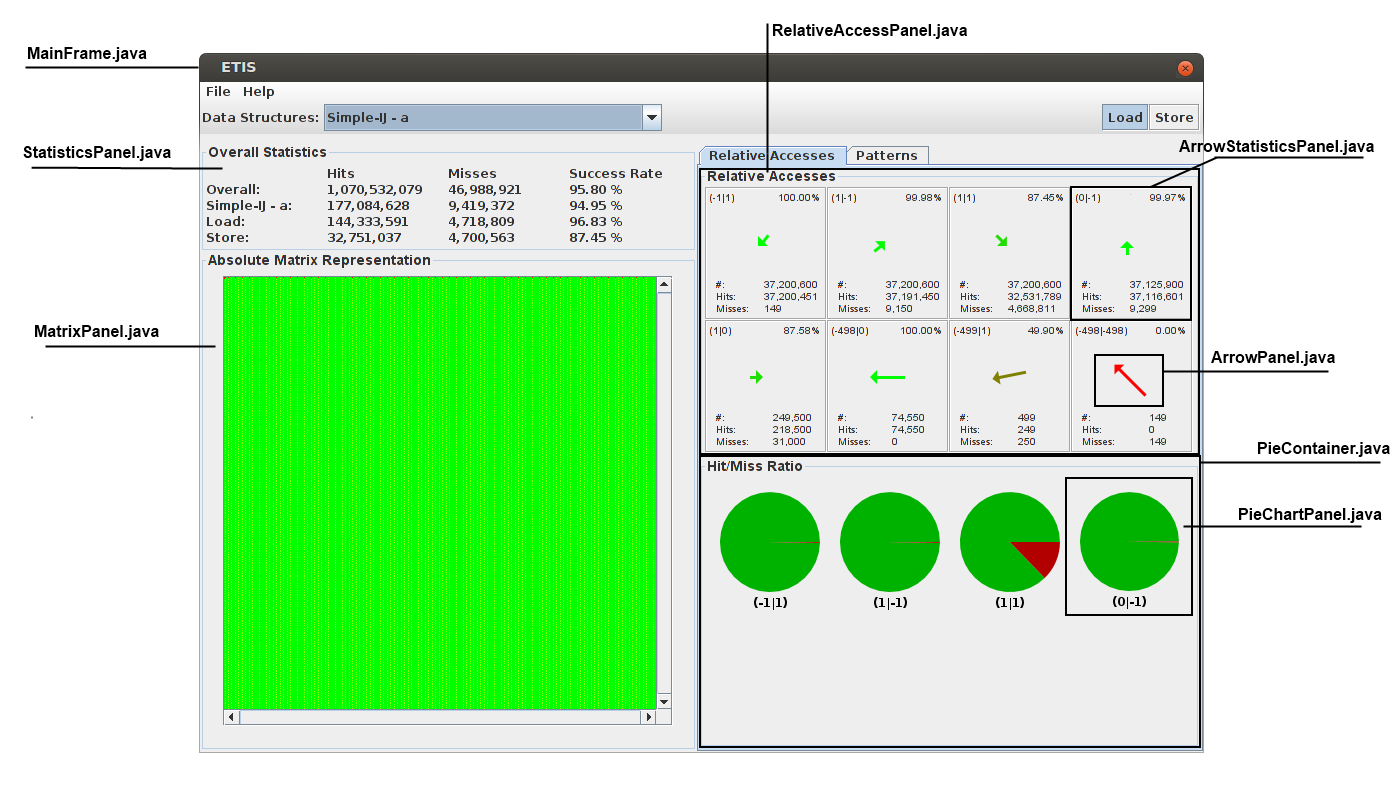
\includegraphics[angle=90,height=700px]{gui/classresp1.png}
\subsection{Informal Class Diagramm}
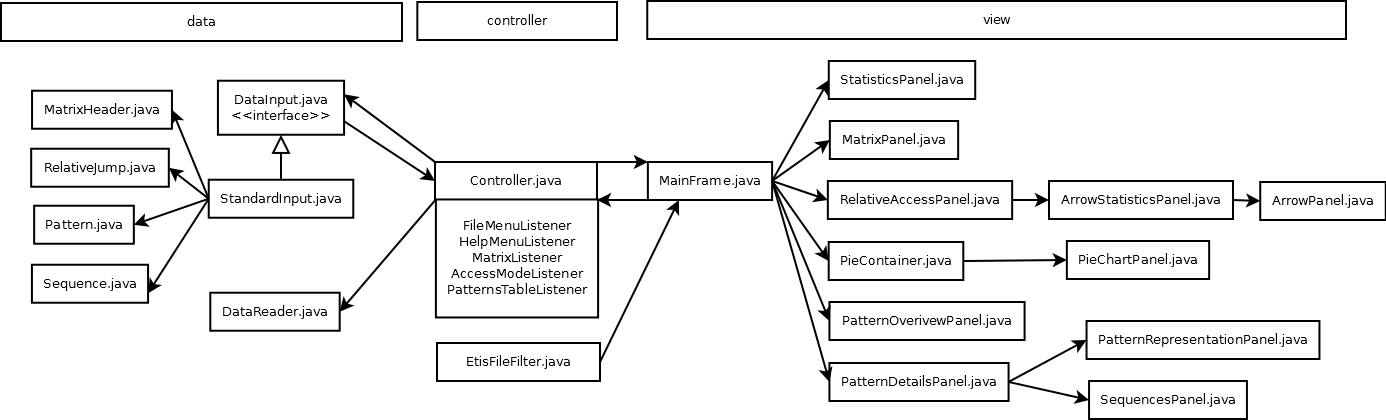
\includegraphics[angle=90,height=560px]{gui/comm.png} 
\subsection{Absolute Matrix Representation} The Absolute Matrix Representation shows the cache usage for each memory cell. Every memory cell is represented by a scaled pixel which is colored as follows:
\begin{description}
\item[white]There has been no access.
\item[red]All accesses have been misses.
\item[green]All accesses have been hits.
\item[other colors between red and green (e.g. yellow)]different hit/access ratios (scaled linearly)
\end{description}
To keep the information readable, the panel showing the matrix has to be zoomable and consequently movable.

\subsubsection{Affine Transformation}
An affine transformation is equivalent to a linear transformation followed by a translation\footnote{\url{http://en.wikipedia.org/wiki/Affine_transformation}}, i.e. it preserves collinearity, parallelism and ratios of colinear points. Here, it is used to adjust the pixels to the current zoom level and position.

Two affine transformations (one for translation, one for scaling) are concatenated to form the affine transformation, which can be used to transform the $(x,y)$-based point values into the actual drawing coordinates.\\

$\underbrace {\left(
   \begin{array}{ccc}
     1 & 0 & scale*d_{x} \\
     0 & 1 & scale*d_{y} \\
     0 & 0 & 1
   \end{array}
\right)}_{Translation}*\underbrace {\left(
   \begin{array}{ccc}
     scale & 0 & 0 \\
     0 & scale & 0 \\
     0 & 0 & 1
   \end{array}
\right)}_{Scaling}=\left(
   \begin{array}{ccc}
     scale & 0 & scale*d_{x} \\
     0 & scale & scale*d_{y} \\
     0 & 0 & 1
   \end{array}
\right)$
\begin{description}
\item[$scale$]actual pixel size
\item[$d_{y}$]offset in x direction
\item[$d_{y}$]offset in y direction
\end{description}


\subsubsection{Implementation}
The Absolute Matrix Representation is implemented in \texttt{view.MatrixPanel} which extends Java's \texttt{JPanel}.

Zooming is enabled by implementing a \texttt{MouseWheelListener} and the \\
\texttt{zoom(MouseWheelEvent e)} method. A new scale is calculated, the scrollbars are adjusted and revalidated. The program also checks that zooming does not result in white space appearing, hence it checks for the view area to only show (parts of) the matrix. Eventually, a repainting is initiated. 

Scrolling is enabled by a \texttt{JScrollPane}. A \texttt{AdjustmentListener} checks for changes to the scrollbar positions and initiates a repainting, where the new $d_{x}$ and $d_{y}$ values will be calculated, as well.

The repainting results in the \texttt{paintComponent(Graphics g)} method getting called. The affine transformation is implemented by an instance of \\
\texttt{AffineTransform} which gets applied to the \texttt{Graphics2D} object. Afterwards, each pixel in the visible area is drawn by drawing 1x1 rectangles.
\subsection{*.etis-File Input} The following illustration gives an overview of the different parts
of the gui:

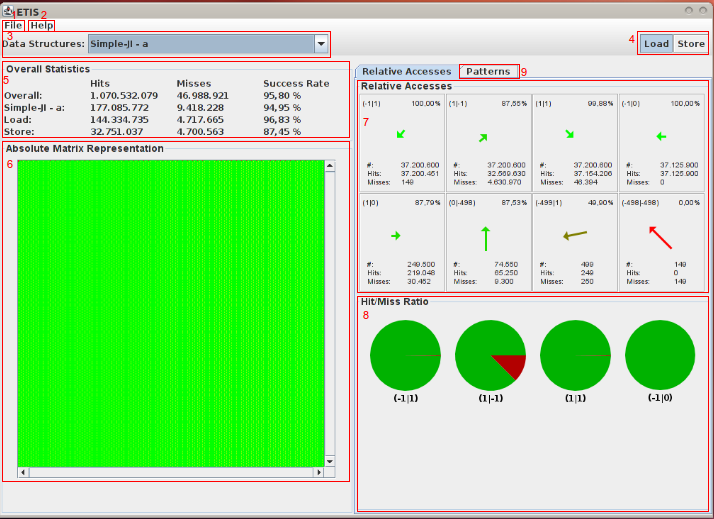
\includegraphics[scale=0.6]{gui/GUIOverview2.png}
\begin{description}
\item [{1$\;$File$\;$Menu:}] Gives you options to a) open a {*}.etis-File
or b) close the application
\item [{2$\;$Help:}] Opens a help menu that can a) show this help text
(Help Contents) b) general information (About)
\item [{3$\;$Data$\;$Structures:}] In the selector right next to this
label, one can select a matrix by name, for which all of the information
gathered by McTracer should be shown.
\item [{4$\;$Load/Store$\;$switch:}] This switch is located in the top
right corner and determines if the information displayed throughout
the rest of the GUI refers to load or store type accesses.
\item [{5$\;$Overall$\;$Statistics:}] This part presents statistics for
the total number of hits/misses and the ratio hits/(hits+misses) aka
success rate for a) all the matrices contained in the selected file
(Overall) b) the selected matrix (by matrix name) c) for load type
accesses on this matrix (Load) d) for store type accesses on this
matrix (Store).
\item [{6$\;$Absolute$\;$Matrix$\;$Representation:}] This part visualizes
the accesses (that is loads or stores as selected by the load/store
switch) that happened on the matrix on a per field basis. Each field
is coloured on a scale from red to green, where red means that 0\%
of the accesses on this field where hits, whereas green means that
100\% of the accesses where hits. This colour scheme is also used
throughout the rest of the graphics appearing in this GUI.
\item [{7$\;$Relative$\;$Accesses:}] In this part the single accesses
(that is loads or stores as selected by the load/store switch) on
different fields are classified by the difference in position of two
consecutive accesses. For example, if the program makes two consecutive
accesses to the fields at positions (1|1) and (1|3) this will give
a new relative access class identified by the position delta of (0|2).
The following information is displayed for the 8 access classes that
were found most often: The number of hits and misses that occurred
for accesses belonging to that class, the corresponding hit/miss ratio
and a graphical representation of the access' position delta with
an arrow. These arrows are coloured in accordance to the hit/miss
ratio. 
\item [{8$\;$Hit/Miss$\;$Ratio:}] In the area the hit/miss ratio for
each relative access is visualized with a pie chart. The area of each
pie chart corresponds to the overall number of accesses that where
found for this relative access compared to the others. That means
an access with a lot of accesses will have a big chart, while an access
with fewer accesses will have a smaller pie chart. It can happen that
some of the accesses do not appear as a pie chart, because their charts
would be too small to be displayed.
\item [{9$\;$Patterns:}] A pattern groups multiple relative accesses in
to bigger sequences in order to give the user a feel of how the matrix
is traversed by the program. By selecting a pattern from the list,
the following detail information is shown below the pattern list:
Each pattern consists of a number of relative accesses that are traversed
in the displayed order. Also for each pattern the total number of
occurrences and the number of hits and misses is presented to the
user. Each pattern is graphically represented by a picture showing
a start point and an arrow for each consecutive relative access. Again
the colouring of the arrows correlates to the hit/miss ratio. The
bottom part shows a list of sequences, of which this pattern is part
of. Patterns do not distinguish load and store.
\item [{10$\;$Sequences}] (Part of patterns tab, not visibile in the preceeding
illustration): A sequence is basically a repetition of a certain pattern.
It displays how often the pattern in question was repeated and which
relative access did \"{}break\"{} the sequence,
that means which relative access was the first one that did not belong
to the pattern. For this relative access the delta in x and y position
is shown. Sometimes the program can recognize a pattern that directly
follows the repetition of the pattern corresponding to the sequence.
If this is the case, this following pattern is identified by the id
as assigned in the pattern list. Of course the same sequence can appear
multiple times, so the number of occurrences of that sequence is shown.\end{description}



\end{document}
